
\documentclass[times]{TRR}
\usepackage{algpseudocode}
\usepackage{algorithm}
\usepackage{graphicx}
\usepackage[affil-it]{authblk}
\usepackage[paperheight=6in,
   paperwidth=5in,
   top=10mm,
   bottom=20mm,
   left=10mm,
   right=10mm]{geometry}
\newcommand\BibTeX{{\rmfamily B\kern-.05em \textsc{i\kern-.025em b}\kern-.08em
T\kern-.1667em\lower.7ex\hbox{E}\kern-.125emX}}
\graphicspath{ {./images/} }
\def\volumeyear{2022}
\begin{document}

\runninghead{}

\title{Conjugate Gradient Solver using Additive Schwarz preconditioner}

\author{Ziya Mammadov, ziya@ut.ee}
\affil{Institute of Computer Science, University of Tartu}

\begin{abstract}
The domain decomposition methods are iterative methods for the solution of linear and non-linear systems and they are mostly used as preconditioners for iterative methods such as GMRES, Conjugate Gradient(CG), etc.  Therefore, Conjugate Gradient solver implementation can be improved by applying different preconditioners by splitting our domain matrix into subdomains which will also make it suitable for extra parallelism. In order to see the benefits that preconditioners might bring Additive Schwarz preconditioner will be applied to the existing CG solver which is written using C and OpenCL programming languages. This report will give a short overview of GPGPU(OpenCL) programming, domain decomposition methods, and their usage in the implementation of the solver.
\end{abstract}

\maketitle

\section{1. Introduction}
In recent years, the convergence properties of algorithms have been explored a lot.
In scientific computing Conjugate Gradient method is used to solve linear equations
$Ax = b$ with large sparse matrices such as the Helmholtz equation. Here $A$ is a symmetric positive- define matrix. The domain decomposition methods are used to reduce the memory consumption used in solving huge problems and to make the computation process faster. The basic idea behind domain decomposition is to partition the domain into small pieces. After partitioning, subdomains can be used to solve the same problem which consumes less memory and also can be used in to solve the problem in parallel. Most of the time domain decomposition methods are used as preconditioners in the iterative solvers to obtain better convergence. An additive Schwarz preconditioner is one of the domain decomposition methods that decrease the condition number of the matrix to faster the range of the convergence. 

\section{2. Conjugate Gradient method}
The conjugate Gradient method is used to optimize a quadratic convex function. The convex optimization problem in quadratic form can be written as:
\begin{center}
$f(x) = 1/2x^{T}Ax - b^{T}x + c$
\end{center}
Here $A$ is matrix $x$ and $b$ are vectors and $c$ is scalar. If we consider that A is symmetric and positive define $f(x)$ can be minimized by the solution (Figure 1):
\begin{center}
$Ax=b$  
\end{center}

\begin{algorithm}
\caption{ Conjugate Gradient}\label{alg:cap}
\begin{algorithmic}
\Ensure $A$ is a symmetric positive-define matrix
\State $r \gets b - Ax$
\State $d \gets r$
\State $\delta \gets r^{T}r$
\While{not converged}
\State $q \gets Ad$
\State $\alpha \gets \dfrac{\delta}{d^{T}q}$
\State $x \gets x + \alpha d$
\State $r \gets r - \alpha q$
\State $\delta_{old} \gets \delta$
\State $\delta \gets r^{T}t$
\State $\beta \gets \dfrac{\delta}{\delta_{old}}$
\State $d \gets r + \beta d$
\EndWhile
\State \Return x
\end{algorithmic}
\end{algorithm}
\begin{par}
The Conjugate gradient method(algorithm 1) is well-known for its iterative behavior using the Krylov subspaces to replace matrix-matrix multiplication with matrix-vector multiplication when the system is large and sparse but the matrix is SPD(symmetric positive-define). The linear combination of $b, Ab,..., A^{j-1}b$ form Krylov subspace $K_j(A,b)$. The algorithm chooses the best $x_j$ from each subspace where the residual $r_j = b - Ax_j$ is orthogonal to $K_j(A,b)$.
\end{par}
\begin{par}
The rate of convergence is dependent on the condition number. A larger condition number $k(A)$ leads to slower convergence. Therefore we can apply preconditioners to our system $M^{-1}(Ax - b) = 0$ where the $k(M^{-1}A) < k(A)$
\end{par}
\begin{figure}[h]
    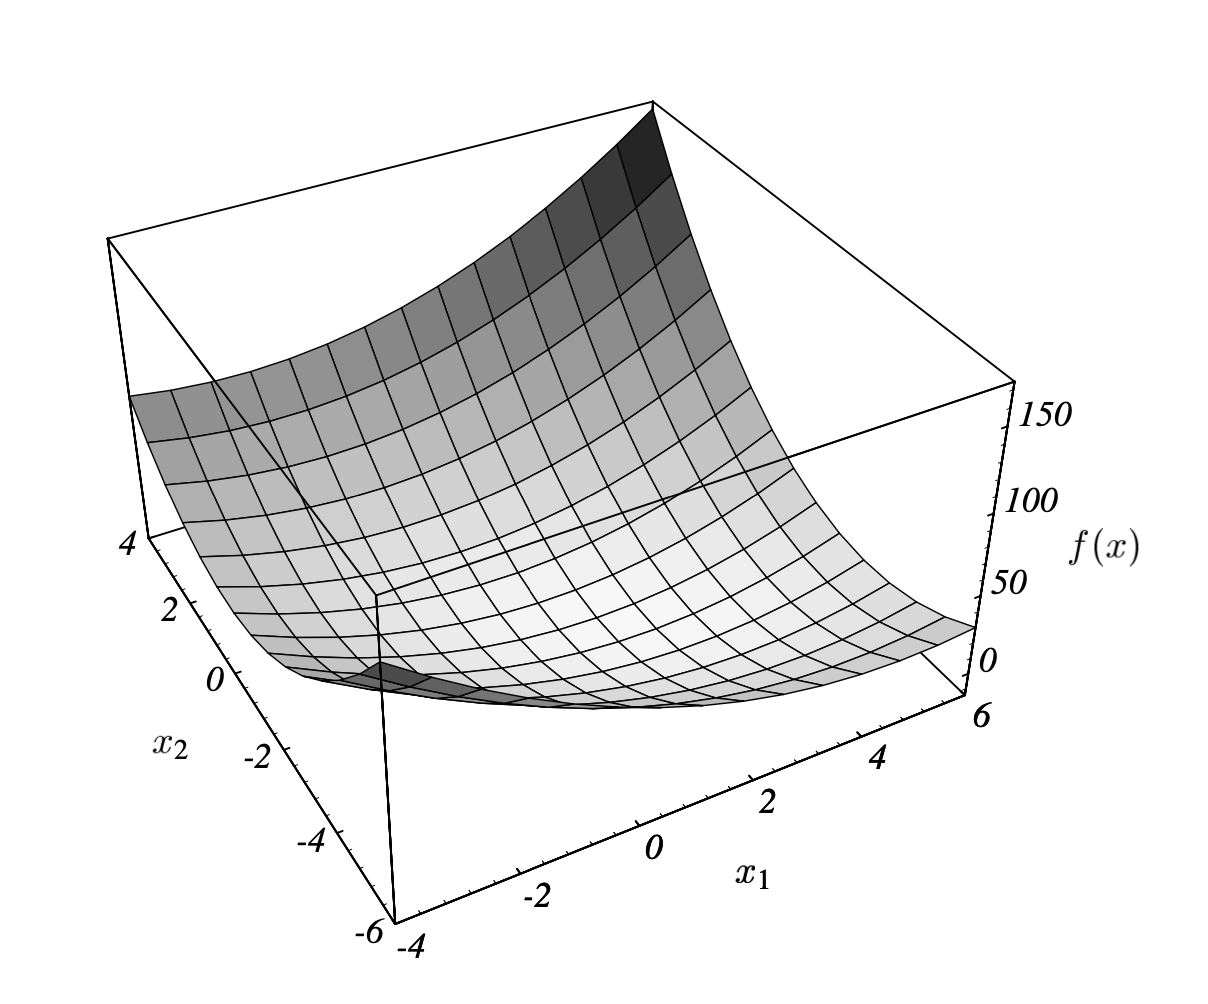
\includegraphics[scale=0.4]{images/quadratic-form-graph.png}
    \caption{The graph of quadratic form $f(x)$. The solution of the $Ax = b$ gives the minimum point to the surface}
\end{figure}
\section{3. General-purpose computing on GPU(GPGPU)} 
\noindent
In the past years, there has been a significant increase in the performance of the graphical processing units. Although they are initially designed for fast image rendering of graphical applications, nowadays GPUs are also widely used for non-graphical applications so-called GPU computing. These improvements give us a chance to write highly parallel programs and make use of their benefits of them. GPU's architecture allows us to run a huge number of threads in parallel with the power of many-core rather than using CPUs which usually have 4 to 8 cores. Therefore, many scientific computations can be accelerated with the help of General-Purpose computing on the GPU(GPGPU). The introduction of a new application programming interface CUDA(Compute Unified Device Architecture) by Nvidia in 2007 gave developers a huge advantage in having large computation in GPUs and pushed GPU computing utilization to the next level. The flaw in CUDA was that it is supported only on Nvidia hardware. Eventually, OpenCl is introduced to support diverse compute devices including Nvidia, AMD, and Intel hardware.
\section{3.1 The main concepts of OpenCl} 
\begin{figure}[h]
    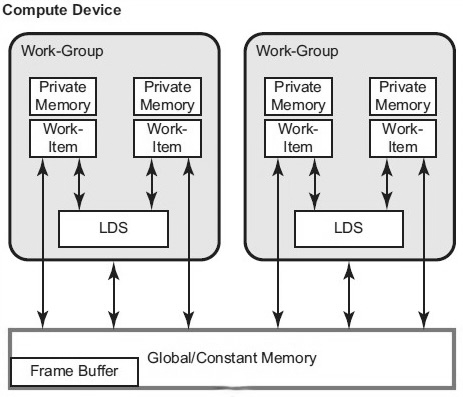
\includegraphics[scale=0.45]{images/memory-model-opencl.png}
    \caption{OpenCl memory model. LDS is an abbreviation for Local data storage}
\end{figure}
The development in OpenCl programs starts with finding the appropriate compute devices in our machines such as a CPU or GPU. The core of compute device is the compute units that can run a set of jobs to achieve great parallelism. The compute units have their own local storage. For instance, a Radeon R5 GPU has 32KB of local memory for each of its compute units. Moreover, every CU consists of multiple processing elements which have their own private memory and this private memory can be accessed only by one work item (thread), however, work items can read from or write to global memory. In OpenCL programs, the host device sends commands from a host to compute device through command queues and these commands are mainly kernel execution or data transfers. Compute device executes each command in the same order as they were in the command queue. The group of work items in the work group is referred to as a wavefront. Typically one workgroup is assigned to one compute unit. Whenever it comes to execution, the wavefront is sent to the compute unit, and each work item inside the same wavefront is run in parallel and in lock-step fashion. However, different wavefronts in a workgroup are executed sequentially. Developers need to know the number of processing elements in the cores for the used device in order to distribute work items into wavefront, although OpenCl is vendor independent in the choice of a computing device. The term NDRange is used to specify the number of work items created for the compute device. NDRange is an N-dimensional array in which each work item is assigned to one index of the array. Specializations of a compute device should be considered while creating NDRange as the devices cannot process work items surpassing the number of processing units. Kernels will be duplicated according to NDRange when the kernel is sent to a computing device and each copy of the kernel will correspond to a work item.
\section{4. Domain Decomposition methods}
\textbf{Domain Decomposition methods} 
Domain decomposition methods are used to make the algorithms run in parallel and fast for linear or nonlinear equations. Domain decomposition implies splitting the domain into approximately equal size subdomains for the single processes. Single program multiple data(SPMD) paradigm is an example of domain decomposition. SPMD executes a single program independently using multiple separate portions of data. It is commonly used in parallel programming in the following cases:
\begin{itemize}
    \item \textbf{MPI} Message passing interface run SPMD on a distributed-memory systems
    \item \textbf{Kernels} run SPMD within a GPU
    \item \textbf{POSIX threads} run SPMD in a shared memory system
\end{itemize}
We can classify the domain decomposition methods as overlapping and non-overlapping. In non-overlapping methods, the subdomains intersect only on their interface. Balancing domain decomposition can be an example of such a method. However, in overlapping methods, the subdomains overlap in one or more interfaces. They are mostly used as preconditioners for iterative methods such as Conjugate Gradient, GMRES, etc. 
\section{4.1 Additive Schwarz}
After many analyses on the Conjugate Gradient method, it has been known if any preconditioner is applied to the system decreasing the condition number, we can still improve the convergence by decreasing the condition number of the new matrix where the preconditioner is applied and we get a same approximate result. Additive Schwarz is one of the preconditioners that is used to decrease the condition number and split the domain into subdomains. We should also not forget that the newly obtained matrix should be symmetric in order for the Conjugate Gradient method to work correctly.

\section{Implementation and optimizations}
Implementation of the Conjugate Gradient method is done by Kert Tali using C and OpenCL. Mentioned code supports CG both for real and complex numbers for more than one right-hand side RHS although there is no native support for the complex numbers in OpenCL. Different kernels have been written in order to gain speed up using the power of GPU. The dot product, sparse matrix-vector multiplication is the main kernel where the parallelism is done. A sparse matrix is a matrix in which only a small portion of the values are non-zero. The coordinate(COO) format is used to store the sparse matrices. This format uses 3 arrays to store the values and their positions(Figure 3).
\begin{figure}[h]
    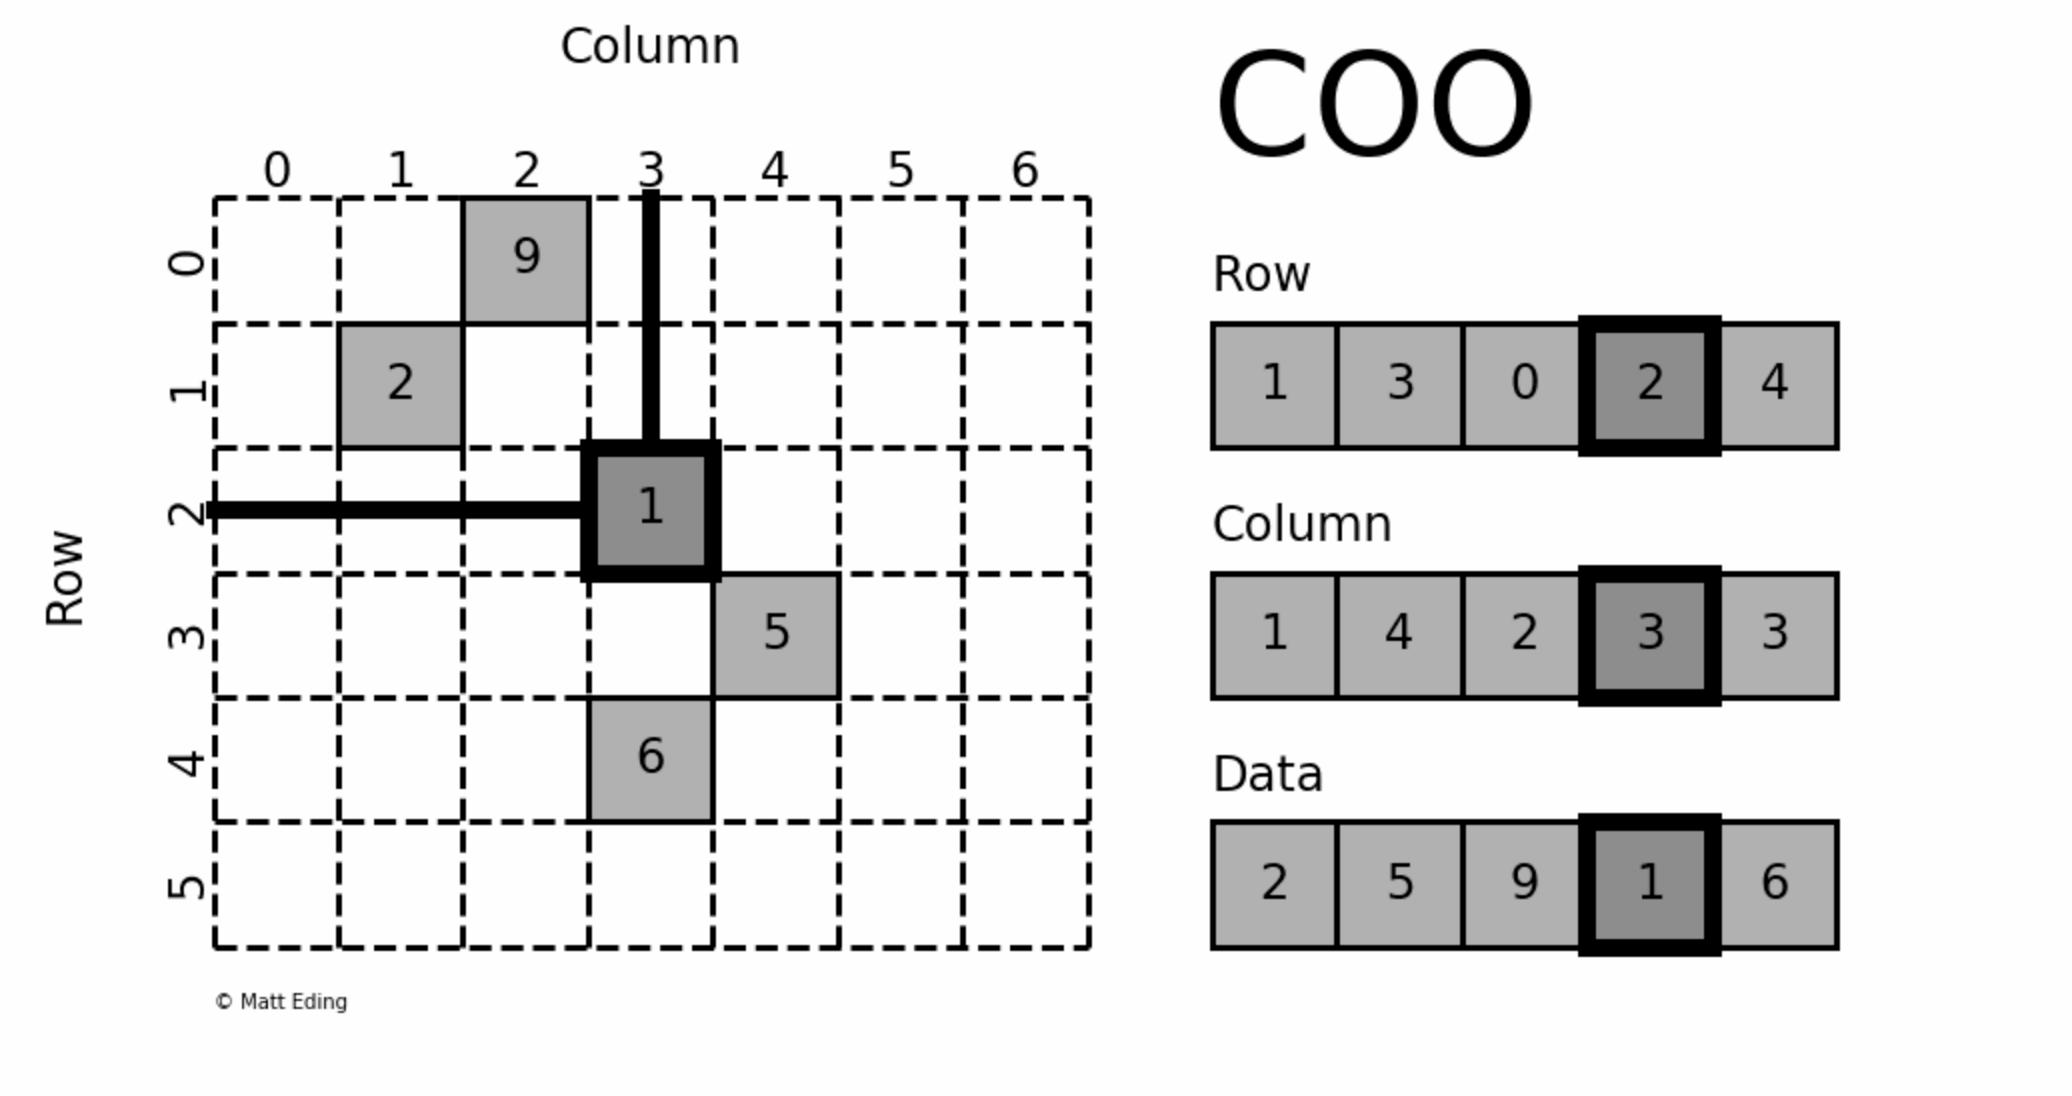
\includegraphics[scale=0.1]{images/coo-format.png}
    \caption{Sparse matrix coordinate format}
\end{figure}
\begin{par}
Implementation of the solver has 2 main parts: 
\begin{itemize}
    \item \textbf{Kernels} - where the BLAS operations are implemented.
    \item \textbf{Device memory management} - it is the host code where the memory allocations are done and kernels are called.
\end{itemize}
The part where the 1-level Schwarz preconditioner is applied is written in Python and submatrices which are the result of preconditioners are sent to the CG function written in C using the python library called \emph{ctypes}. It uses the shared library to find the correct function.
\end{par}
\section{Evaluation}
The conjugate gradient implementation in c and OpenCL has been compared with the clSPARSE OpenCL library that has a CG solver for real-valued input. I couldn't benchmark the preconditioned Conjugate Gradient method due to time limitations and the lack of knowledge in C and OpenCL. Although the matrices with very small dimensions worked when the CG function was called from python, matrices with bigger dimensions gave wrong results. The solver written in C needs to be debugged in order to find the problem leading to the incorrect result.
\section{Future work}
The Conjugate Gradient implementation needs to be deeply debugged. After debugging and fixing the problem, we can compare the performance of general CG and preconditioned CG. Moreover, some other preconditioners such as 2-level Additive Schwarz can be applied to CG to improve the performance.
\begin{thebibliography}{99}


\bibitem{R1}
Shewchuk, J.R., 1994. An introduction to the conjugate gradient method without the agonizing pain.
\bibitem{R2}
Komatsu, K., Sato, K., Arai, Y., Koyama, K., Takizawa, H., Kobayashi, H. (2010, June). Evaluating performance and portability of OpenCL programs. In The fifth international workshop on automatic performance tuning (Vol. 66, p. 1).
\bibitem{R3}
Van der Vorst, Henk. (2000). Krylov Subspace Iteration. Computing in Science & Engineering. 2. 32-37. 10.1109/5992.814655. 
\bibitem{R4}
Thompson, Jonathan A. and Kristofer Schlachter. “An Introduction to the OpenCL Programming Model.” (2012).
\bibitem{R5}
J. Fang, A. L. Varbanescu and H. Sips, "A Comprehensive Performance Comparison of CUDA and OpenCL," 2011 International Conference on Parallel Processing, 2011, pp. 216-225, doi: 10.1109/ICPP.2011.45.
\bibitem{R6}
Peng Du, Rick Weber, Piotr Luszczek, Stanimire Tomov, Gregory Peterson, Jack Dongarra,
From CUDA to OpenCL: Towards a performance-portable solution for multi-platform GPU programming,
Parallel Computing, Volume 38, Issue 8,2012, Pages 391-407, ISSN 0167-8191
\bibitem{R7}{Liu, Hui, et al. "Development of a restricted additive Schwarz preconditioner for sparse linear systems on NVIDIA GPU." International Journal of Numerical Analysis and Modelling: Series B 5.1-2 (2014): 13-20.}
\end{thebibliography}
\end{document}
